\documentclass{beamer}
\usetheme{teamhenkler}

% ==========================
% Packages
% ==========================

\usepackage{chngcntr}
\usepackage{bbm}
\usepackage{xargs}  

% ==========================
% Math Packages
% ==========================

\usepackage{amsmath, amssymb, amsfonts, mathtools}
\usepackage{algorithm}
\usepackage{amsthm}
\usepackage{algpseudocode}
% ==========================
% Graphic Packages
% ==========================
\usepackage{tikz}
\usepackage{tikz-cd}
\usepackage{tikz-3dplot}
\usepackage{xcolor} % For modern color palette
\usepackage{graphicx}
\usepackage{subcaption}
\usepackage{pgfplots}
\usepackage[most]{tcolorbox}
% ==========================
% Tikz Libraries
% =========================
\usetikzlibrary{positioning}
\usetikzlibrary{ arrows.meta}
\usetikzlibrary{shapes.geometric}
\usetikzlibrary{calc}
\usetikzlibrary{arrows}
\usetikzlibrary{shapes, arrows, positioning, fit, calc, backgrounds, chains,decorations.pathreplacing,hobby}
\usetikzlibrary{mindmap,trees}
\usetikzlibrary{automata,positioning}
\usetikzlibrary{decorations.markings}
% ==========================
% Pfg Libraries
% =========================
\usepgfkeyslibrary{ext.pgfkeys-plus}
\usepgfplotslibrary{groupplots}
\pgfplotsset{compat=1.17,colormap/viridis}

% ==========================
% Document Settings
% ==========================

%\addto\captionsenglish{\renewcommand{\bibname}{Bibliography}}
%\setcounter{secnumdepth}{5}
%\setcounter{tocdepth}{1}


% ==========================
% Reference Settings
% ==========================

\newcommand{\secref}[1]{Section \ref{#1}}
\newcommand{\chapref}[1]{section \ref{#1}}
\newcommand{\figref}[1]{Fig \ref{#1}}
\newcommand{\equaref}[1]{(\ref{#1})}
\newcommand{\citepaperof}[2]{\textit{#2} in \cite{#1}}
\newcommand{\citepaperofs}[2]{\textit{#2 et al.} in \cite{#1}}
\newcommand{\algoref}[1]{Algorithm \ref{#1}}
\newcommand{\defref}[1]{Definition \ref{#1}}
\newcommand{\tabref}[1]{Table \ref{#1}}
\newcommand{\ruleref}[1]{Rule \ref{#1}}
\newcommand{\subfigref}[1]{(\subref{#1})} 
\newcommand{\appref}[1]{Appendix \ref{#1}}
\newcommand{\sectionbreak}{\clearpage}


% ==========================
% Theorem Style
% ==========================

%\theoremstyle{definition}
%\newtheorem{definition}{Definition}
%
%\theoremstyle{definition}
%\newtheorem{statecomprule}{SC-Rule}
%
%\theoremstyle{definition}
%\newtheorem{norm}{Norm}

% ==========================
% Colors
% ==========================
\definecolor{viridisgreencolor}{RGB}{32, 162, 57} % Viridis green color
\definecolor{viridisorangecolor}{RGB}{253, 174, 97}
\definecolor{viridisbluecolor}{RGB}{68, 1, 84}
\definecolor{viridisyellowcolor}{RGB}{253, 231, 37}
\definecolor{viridispurplecolor}{RGB}{108, 60, 142}
\definecolor{viridiscyancolor}{RGB}{1, 133, 113}
\definecolor{viridismagentacolor}{RGB}{177, 3, 155}


\definecolor{layer1}{HTML}{4CAF50} % Green for perception layer
\definecolor{layer2}{HTML}{2196F3} % Blue for network layer
\definecolor{layer3}{HTML}{FFC107} % Yellow for computation layer
\definecolor{layer4}{HTML}{F44336} % Red for control layer
\definecolor{layer5}{HTML}{9C27B0} % Purple for application layer
\definecolor{subLayer1}{HTML}{388E3C} % Darker green for sublayer 1
\definecolor{subLayer2}{HTML}{66BB6A} % Lighter green for sublayer 2


% ==========================
% Tikkz styles
% ==========================

\tikzstyle{layer} = [rectangle, rounded corners, text centered, draw=black!50, dashed, inner sep= 15pt]
\tikzstyle{layerTight} = [rectangle, rounded corners, minimum width=6.3cm, minimum height=1cm, text centered, draw=black!50, dashed, inner sep= 5pt]
\tikzstyle{layerGroup} = [rectangle, rounded corners, minimum width=7.3cm, minimum height=1cm, text centered, draw= black, dashed, inner sep= 5pt]
\tikzstyle{subLayer} = [rectangle, rounded corners, minimum width=2.8cm, minimum height=3cm, text centered, draw=black]
\tikzstyle{arrow} = [thick,->,>=stealth]
\tikzstyle{arrowDown} = [thick,<-,>=stealth]
\tikzstyle{doublearrow} = [thick,<->,>=stealth]
\tikzstyle{title} = [font=\color{black}\fontsize{9}{9}\selectfont, opacity=0.5]
\tikzset{arrowstyle/.style={draw=black, fill=layer5!30, single arrow,single arrow,
		single arrow head extend=.4cm,}}
\newcommand{\asymcloud}[2][.1]{%Cloud shape
	\begin{scope}[#2]
		\pgftransformscale{#1}%    
		\pgfpathmoveto{\pgfpoint{261 pt}{115 pt}} 
		\pgfpathcurveto{\pgfqpoint{70 pt}{107 pt}}
		{\pgfqpoint{137 pt}{291 pt}}
		{\pgfqpoint{260 pt}{273 pt}} 
		\pgfpathcurveto{\pgfqpoint{78 pt}{382 pt}}
		{\pgfqpoint{381 pt}{445 pt}}
		{\pgfqpoint{412 pt}{410 pt}}
		\pgfpathcurveto{\pgfqpoint{577 pt}{587 pt}}
		{\pgfqpoint{698 pt}{488 pt}}
		{\pgfqpoint{685 pt}{366 pt}}
		\pgfpathcurveto{\pgfqpoint{840 pt}{192 pt}}
		{\pgfqpoint{610 pt}{157 pt}}
		{\pgfqpoint{610 pt}{157 pt}}
		\pgfpathcurveto{\pgfqpoint{531 pt}{39 pt}}
		{\pgfqpoint{298 pt}{51 pt}}
		{\pgfqpoint{261 pt}{115 pt}}
		\pgfusepath{fill,stroke}         
\end{scope}}    


\newcommand{\defineplane}[7]{%
	% Inputs: right uppermost point (#1, #2, #3), base (#4), height (#5), fill style (#6), vertex names (#7)
	\coordinate (#7-TopRight) at (#1, #2, #3);
	\coordinate (#7-TopLeft) at (#1-#4, #2, #3);
	\coordinate (#7-BottomRight) at (#1, #2-#5, #3);
	\coordinate (#7-BottomLeft) at (#1-#4, #2-#5, #3);
	\coordinate (#7-MiddlePoint) at (#1/4+#1/4-#4/4+#1/4+#1/4-#4/4,         #2/4+#2/4+#2/4-#5/4+#2/4-#5/4,            #3);
	
	% Draw the plane
	\filldraw[#6] (#7-TopRight) -- (#7-TopLeft) -- (#7-BottomLeft) -- (#7-BottomRight) -- cycle;
	\draw[thick] (#7-TopRight) -- (#7-TopLeft) -- (#7-BottomLeft) -- (#7-BottomRight) -- cycle;
	\node[fill=none, circle, inner sep=0pt] (#7-MiddlePoint) at (#7-MiddlePoint) {}; 
	
	% Automatically define the anchor points for the plane (center of each edge)
	\coordinate (#7-west) at ($(#7-TopLeft)!0.5!(#7-BottomLeft)$);   % west anchor at the center of the left edge
	\coordinate (#7-east) at ($(#7-TopRight)!0.5!(#7-BottomRight)$);  % east anchor at the center of the right edge
	\coordinate (#7-north) at ($(#7-TopLeft)!0.5!(#7-TopRight)$);    % north anchor at the center of the top edge
	\coordinate (#7-south) at ($(#7-BottomLeft)!0.5!(#7-BottomRight)$);  % south anchor at the center of the bottom edge
	
}



\tikzdeclarecoordinatesystem{hexaring}{%
	\pgfqkeys{/tikz/cs}{#1}%
	\pgfmathtruncatemacro\hRing{\pgfkeysvalueof{/tikz/cs/ring}}%
	\ifnum\hRing=0 \pgfpointorigin
	\else
	\pgfmathtruncatemacro\hPos{\pgfkeysvalueof{/tikz/cs/pos}}%
	\pgfmathtruncatemacro\hSide{\hPos/\hRing}%
	\pgfmathtruncatemacro\hPosOnSide{mod(\hPos,\hRing)}%
	\pgfpointlineattime{\hPosOnSide/\hRing}
	{\pgfpointpolarxy{30+\hSide*60}{1.73205*\hRing}}
	{\pgfpointpolarxy{90+\hSide*60}{1.73205*\hRing}}%
	\fi}
\tikzset{
	cs/ring/.initial=0, cs/pos/.initial=0, list/.initial={0,...,4},
	hexagon path/.style 2 args={
		insert path={plot[sharp cycle,samples at={0, 60, ..., 359}](\x:1)}},
	hexagon/.style 2 args={
		hexagon ring #1/.try={#2}, hexagon pos #2/.try={#1},
		/utils/TeX/ifnum={#1=0}{}{
			hexagon not ring 0/.try={#1}{#2},
			style/.pgfmath wrap={hexagon side ##1/.try={#1}{#2}}{int(#2/#1)},
			style/.pgfmath wrap={hexagon pos' ##1/.try={#1}{#2}}{int(mod(#2,#1))}}}}
\newcommand*\tikzhexagonofhexagons[1][]{%
	\foreach[/utils/exec=\tikzset{#1}, expand list,
	evaluate={\hexPerRing=int(max(1,\ring*6)-1);}]\ring in{\pgfkeysvalueof{/tikz/list}}
	\foreach[/tikz/cs/ring=\ring]\pos in {0, ..., \hexPerRing}
	\draw[hexagon={\ring}{\pos}, shift={(hexaring cs: pos=\pos)}, hexagon path={\ring}{\pos}];}


% ==========================
% Boxes for cool definitions, examples etc
% ==========================


\tcbset{
	myboxstyle/.style={
		enhanced, breakable,
		sharp corners,
		left skip=8mm,
		attach boxed title to top left={yshift*=-\tcboxedtitleheight/2},
		boxed title style={colframe=#1!40, height=6mm, bean arc, boxrule=1pt},
		colback=#1!10, colframe=#1!30, boxrule=1pt,
		coltitle=black, colbacktitle=#1!10,
		fonttitle=\bfseries,
		underlay boxed title={%
			\node[circle, fill=#1!10, draw=#1!40, inner sep=1pt, minimum size=6mm, line width=1pt, font=\bfseries] (boxnumber) at ([xshift=-6mm]title.west) {\thetcbcounter};
		},
		underlay unbroken={%
			\draw[#1!40, line width=1pt] (title.west)--(boxnumber);
			\draw[#1!40, -|, line width=1pt] (boxnumber)--(boxnumber|-frame.south);
		},
		underlay first={%
			\draw[#1!40, line width=1pt] (title.west)--(boxnumber);
			\draw[#1!40, line width=1pt] (boxnumber)--(boxnumber|-frame.south);
		},
		underlay middle={%
			\draw[#1!40, line width=1pt] (boxnumber|-frame.north)--(boxnumber|-frame.south);
		},
		underlay last={%
			\draw[#1!40, -|, line width=1pt] (boxnumber|-frame.north)--(boxnumber|-frame.south);
		},
	}
}

% Define the boxed environment
\newtcolorbox{definitionbox}[2][]{%
	colback=white, % Background color
	colframe=black, % Border color
	fonttitle=\bfseries, % Title font
	title=\textbf{Definition \arabic{definitionCounter}}:~\textit{#1}, % Title format
	sharp corners, % Box style
}


\newtcolorbox[use counter=definitionCounter]{definitionBox}[2][]{%
	myboxstyle=blue, title=\textbf{Definition}:~\textit{#2}, #1
}

\newtcolorbox[use counter=exampleCounter]{exampleBox}[1][]{%
	myboxstyle=green, title=\textbf{Example}, #1
}


\newtcolorbox[use counter=assumptionCounter]{assumptionBox}[1][]{%
	myboxstyle=red, title=\textbf{Assumption}, #1
}
\newtcolorbox[use counter=propertyCounter]{propertyBox}[1][]{%
	myboxstyle=cyan, title=\textbf{Property}, #1
}


% ==========================
% Counters
% ==========================


\newcounter{exampleCounter}
\newcounter{definitionCounter}
\newcounter{assumptionCounter}
\newcounter{propertyCounter}


% ==========================
% Useful Command to write notes, missing citations etc
% ==========================
\newcommand{\citationRequired}{\textcolor{red}{(CITATION)}}


\usepackage[colorinlistoftodos,prependcaption,textsize=tiny]{todonotes}
\newcommandx{\unsure}[2][1=]{\todo[linecolor=red,backgroundcolor=red!25,bordercolor=red,#1]{#2}}
\newcommandx{\change}[2][1=]{\todo[linecolor=blue,backgroundcolor=blue!25,bordercolor=blue,#1]{#2}}
\newcommandx{\info}[2][1=]{\todo[linecolor=OliveGreen,backgroundcolor=OliveGreen!25,bordercolor=OliveGreen,#1]{#2}}
\newcommandx{\improvement}[2][1=]{\todo[linecolor=Plum,backgroundcolor=Plum!25,bordercolor=Plum,#1]{#2}}
\newcommandx{\thiswillnotshow}[2][1=]{\todo[disable,#1]{#2}}

\newcommand{\tabitem}{~~\llap{\textbullet}~~}


\newenvironment{missingelements}[1][Missing Elements]
{%
	\begin{tcolorbox}[colframe=red, colback=white, boxrule=1pt, arc=0pt]
		\textbf{\color{red}#1} % Title in bold and red
		\begin{itemize}
		}
		{%
		\end{itemize}
	\end{tcolorbox}
}


\newenvironment{ideastoinclude}[1][Possible ideas]
{%
	\begin{tcolorbox}[colframe=blue, colback=white, boxrule=1pt, arc=0pt]
		\textbf{\color{blue}#1} % Title in bold and red
		\begin{itemize}
		}
		{%
		\end{itemize}
	\end{tcolorbox}
}

\newenvironment{whattocheck}[1][What's there to check]
{%
	\begin{tcolorbox}[colframe=orange, colback=white, boxrule=1pt, arc=0pt]
		\textbf{\color{orange}#1} % Title in bold and red
		\begin{itemize}
		}
		{%
		\end{itemize}
	\end{tcolorbox}
}

\usepackage[utf8]{inputenc}
\usepackage[T1]{fontenc}
\usepackage{longtable}
\usepackage{fancyvrb}

\title{A minimal example}
\date{\today}
\author{author}
\subtitle{Master Thesis}
\email{luca.brodo@hshl.de}

\thset{uni=HSHL,
inner/sectionpage=progressbarHSHL,
outer/footlinestyle=slick, 
outer/progressbar=frametitlestatic,
color/background=light
}



\begin{document}
\maketitle
\maketoc
\begin{frame}{Options to set with \texttt{\textbackslash thset\{\}} command  }
    \begin{table}[h]
        \centering
        \begin{tabular}{|l|l|}
            \hline
            \textbf{Key} & \textbf{Options} \\ 
            \hline
            uni & HSHL, Fhd \\ \hline
            inner/sectionpage & none, simple, \\&progressbar, progressbarHSHL \\ \hline
            inner/subsectionpage & none, simple, progressbar \\ \hline
            color/block & transparent, fill \\ \hline
            color/background & dark, light \\ \hline
            outer/footlinestyle & plain, slick \\ \hline
            outer/numbering & none, counter, fraction \\ \hline
            outer/progressbar & none, head, frametitle, \\& foot, headstatic, \\&frametitlestatic, footstatic \\ \hline
        \end{tabular}
       
    \end{table}
    \end{frame}
    
    \section[Example0]{Talking about a theorem}
    \begin{frame} 
    \frametitle{There Is No Largst Prime Number} 
    \framesubtitle{The proof uses \textit{reductio ad absurdum}.} 
    \begin{theorem}
    There is no largest prime number. \end{theorem} 
    \begin{enumerate} 
    \item<1-| alert@1> Suppose $p$ were the largest prime number. 
    \item<2-> Let $q$ be the product of the first $p$ numbers. 
    \item<3-> Then $q+1$ is not divisible by any of them. 
    \item<1-> But $q + 1$ is greater than $1$, thus divisible by some prime
    number not in the first $p$ numbers. 
    \end{enumerate}
    \end{frame}
  
    
\section[Example 1]{Image next to text }

\begin{frame}{Tackling 4 Main Challenges}
	\begin{columns}
		\begin{column}{0.4\textwidth}
			
			\begin{itemize}
				\item \alert<1>{AV Dispatching}
				\item \alert<2>{AV Routing}
				\item \alert<3>{AV Rebalancing}
				\item \alert<4>{Ride-Sharing and Delivery Pooling}
			\end{itemize}
			
				
		\end{column}
		%%
		\begin{column}{0.6\textwidth}
			\only<1>{ % AV Dispatching image
				\begin{figure}
    \resizebox{0.7\textwidth}{!}{
    \begin{tikzpicture}[>=stealth]
        
        % Define clients nodes
        \node[inner sep=0pt] (client1) at (-3,2.5) {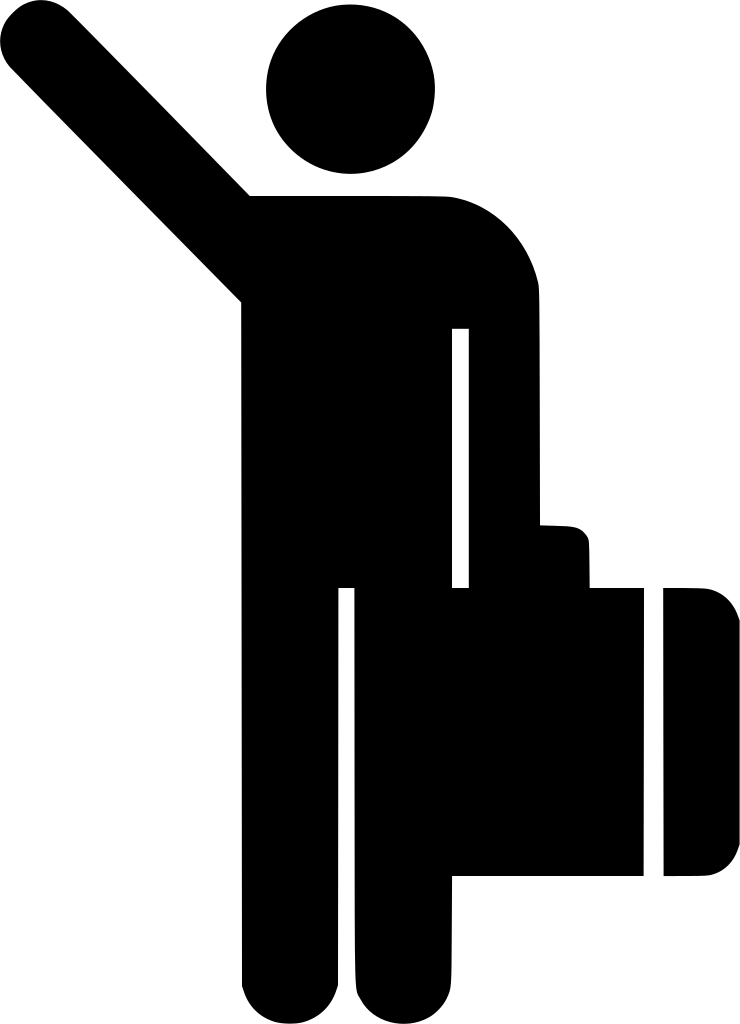
\includegraphics[width=1.1cm]{assets/img/client.png}};
        \node[inner sep=0pt] (client2) at (0,2.5) {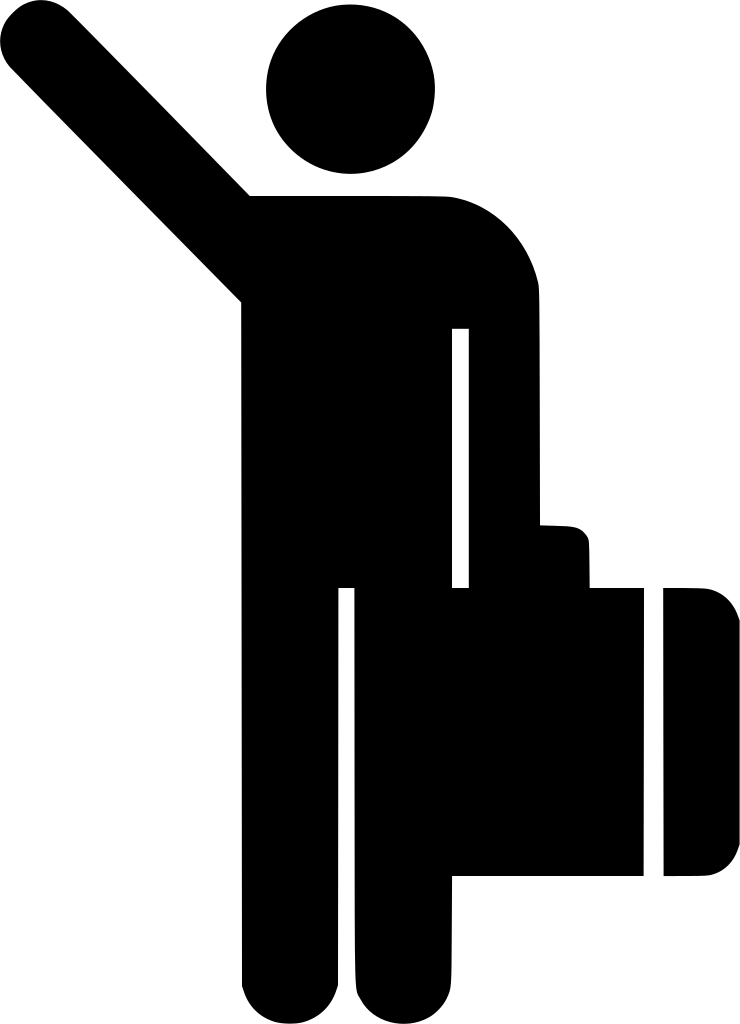
\includegraphics[width=1.1cm]{assets/img/client.png}};
        \node[inner sep=0pt] (client3) at (3,2.5) {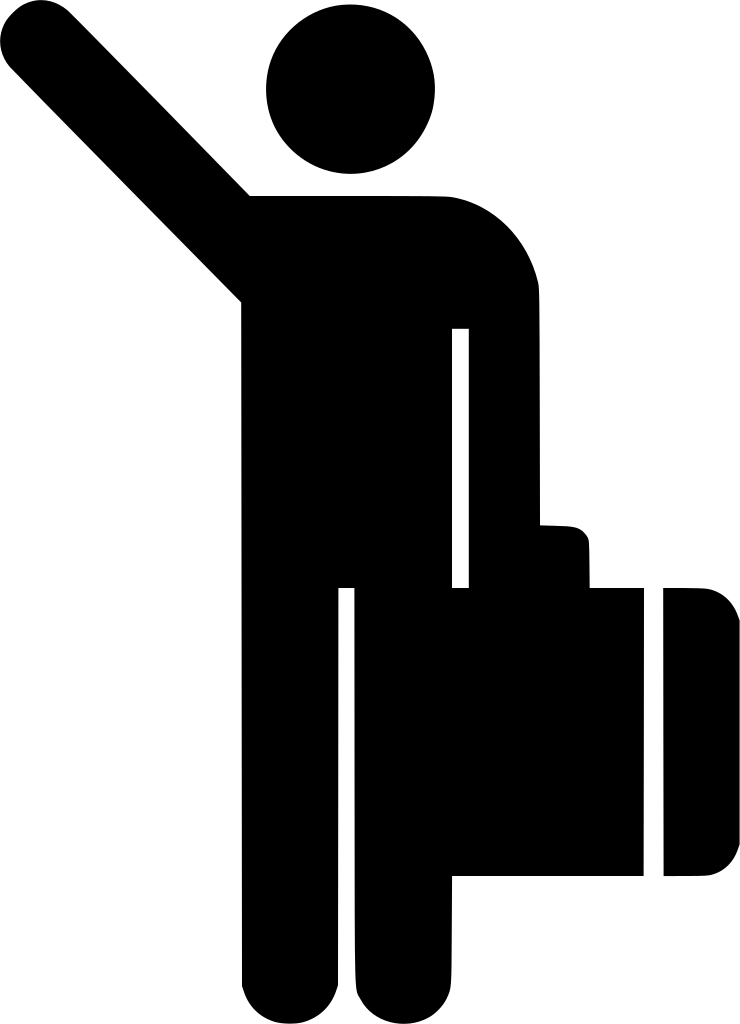
\includegraphics[width=1.1cm]{assets/img/client.png}};
        \node[inner sep=0pt] (client4) at (-4,0) {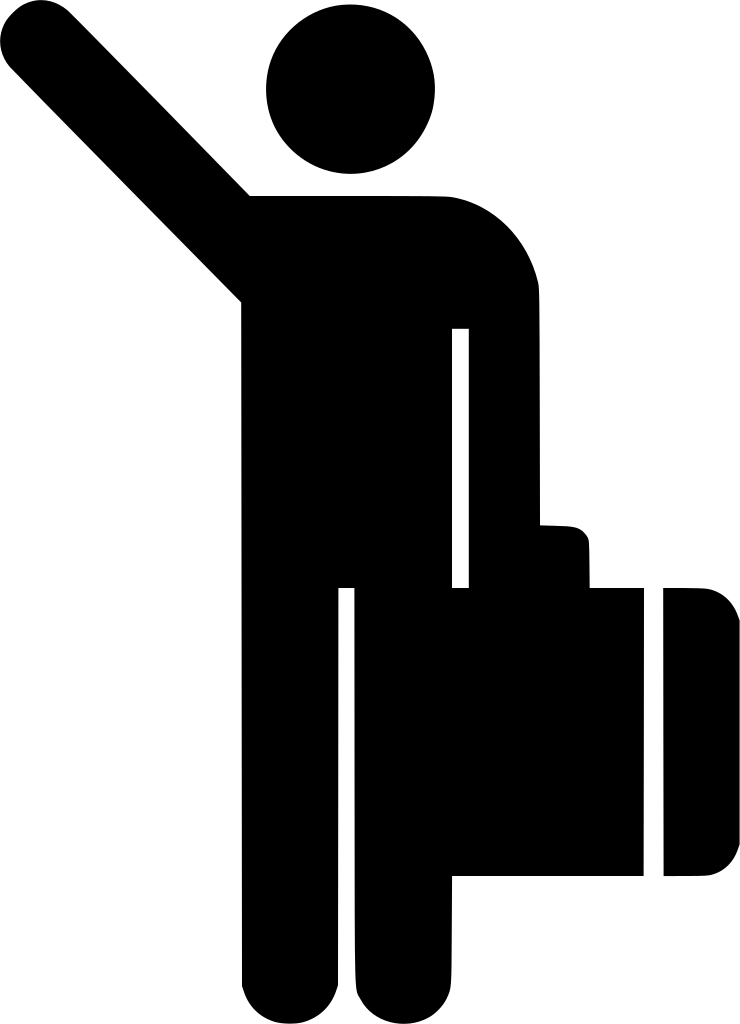
\includegraphics[width=1.1cm]{assets/img/client.png}};
        \node[inner sep=0pt] (client5) at (-1,0) {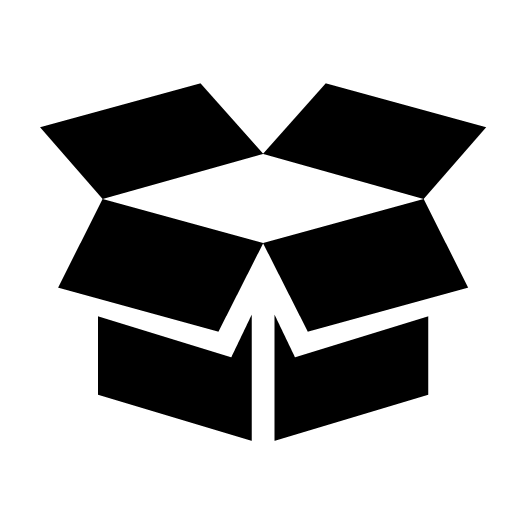
\includegraphics[width=1.1cm]{assets/img/goods.png}};
        \node[inner sep=0pt] (client6) at (1,0) {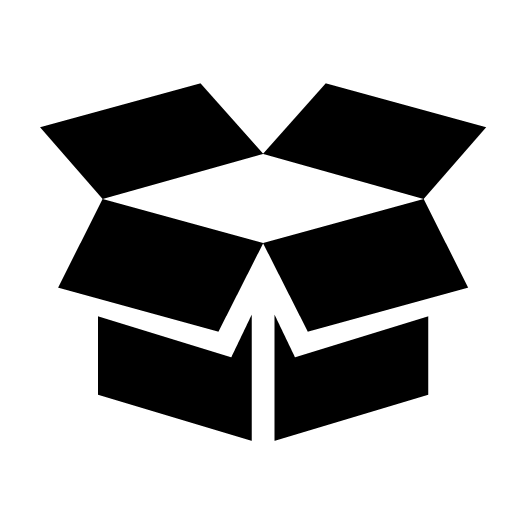
\includegraphics[width=1.1cm]{assets/img/goods.png}};
        \node[inner sep=0pt] (client7) at (4,0) {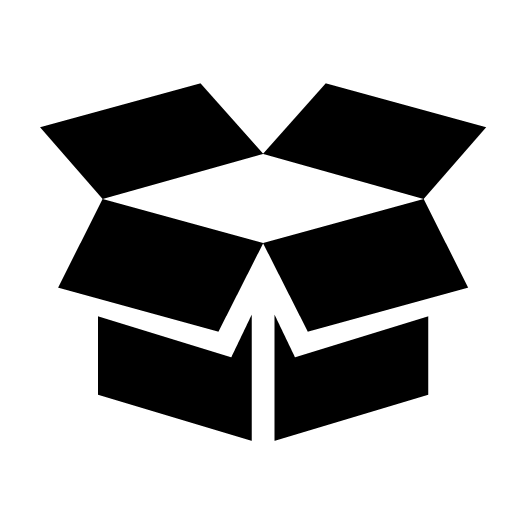
\includegraphics[width=1.1cm]{assets/img/goods.png}};
        
        % Define AVs nodes
        \node[inner sep=0pt] (AV1) at (-3,-3) {
\includegraphics[width=2.4cm]{assets/img/car.png}};
        \node[inner sep=0pt] (AV2) at (0,-3) {
\includegraphics[width=2.4cm]{assets/img/car.png}};
        \node[inner sep=0pt] (AV3) at (3,-3) {
\includegraphics[width=2.4cm]{assets/img/car.png}};

        
        % Arrows from clients to AVs
        \draw[->] (client1.south) -- (AV1.north);
        \draw[->] (client2.south) -- (AV2.north);
        \draw[->] (client3.south) -- (AV3.north);
        \draw[->] (client4.south) -- (AV1.north);
        \draw[->] (client5.south) -- (AV2.north);
        \draw[->] (client6.south) -- (AV2.north);
        \draw[->] (client7.south) -- (AV3.north);
        
        % Label clients and AVs
        \node[above=0.2cm of client1] {Client 1};
        \node[above=0.2cm of client2] {Client 2};
        \node[above=0.2cm of client3] {Client 3};
        \node[above=0.2cm of client4] {Client 4};
        \node[above=0.2cm of client5] {Client 5};
        \node[above=0.2cm of client6] {Client 6};
        \node[above=0.2cm of client7] {Client 7};
        \node[below=0.2cm of AV1] {AV 1};
        \node[below=0.2cm of AV2] {AV 2};
        \node[below=0.2cm of AV3] {AV 3};

        
    \end{tikzpicture}
    
}
\end{figure}
			}
			\only<2>{ % AV Routing image
				\begin{figure}
    \resizebox{0.9\textwidth}{!}{
    \begin{tikzpicture}[>=stealth]
        % Define places nodes
        \node[circle, draw, minimum size=1.5cm] (place1) at (-3,2) { 1};
        \node[circle, draw, minimum size=1.5cm] (place2) at (0,2) { 2};
        \node[circle, draw, minimum size=1.5cm] (place3) at (3,2) { 3};
        \node[circle, draw, minimum size=1.5cm] (place4) at (-4,-1) { 4};
        \node[circle, draw, minimum size=1.5cm] (place5) at (-1,-1) { 5};
        \node[circle, draw, minimum size=1.5cm] (place6) at (1,-1) { 6};
        \node[circle, draw, minimum size=1.5cm] (place7) at (4,-1) { 7};
        
        % Arrows for roads
        \draw[->] (place1) -- (place2);
        %\draw[->] (place2) -- (place3);
        \draw[->] (place1) -- (place4);
        %\draw[->] (place4) -- (place5);
        \draw[->] (place5) -- (place6);
        \draw[->] (place2) -- (place6);
        \draw[->] (place6) -- (place7);
        \draw[->] (place7) -- (place3);
        
        %\draw[->,] (place4) -- (place5) node[midway,above,sloped] {
\includegraphics[width=1cm]{assets/img/car.png} };
        \draw[->] (place4) -- node[midway, above, sloped] {
\includegraphics[width=1cm]{assets/img/car.png}} node[midway, above=0.8cm] {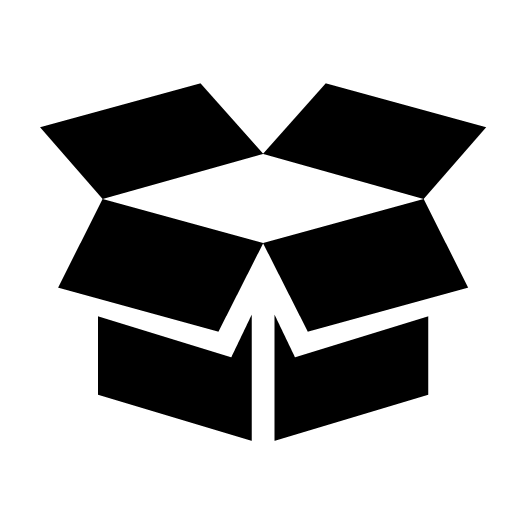
\includegraphics[width=0.5cm]{assets/img/goods.png}} (place5);
        
        %\draw[->,] (place2) -- (place3) node[midway,above,sloped] {
\includegraphics[width=1cm]{assets/img/car.png} };
        \draw[->] (place2) -- node[midway, above, sloped] {
\includegraphics[width=1cm]{assets/img/car.png}} node[midway, above=0.8cm] {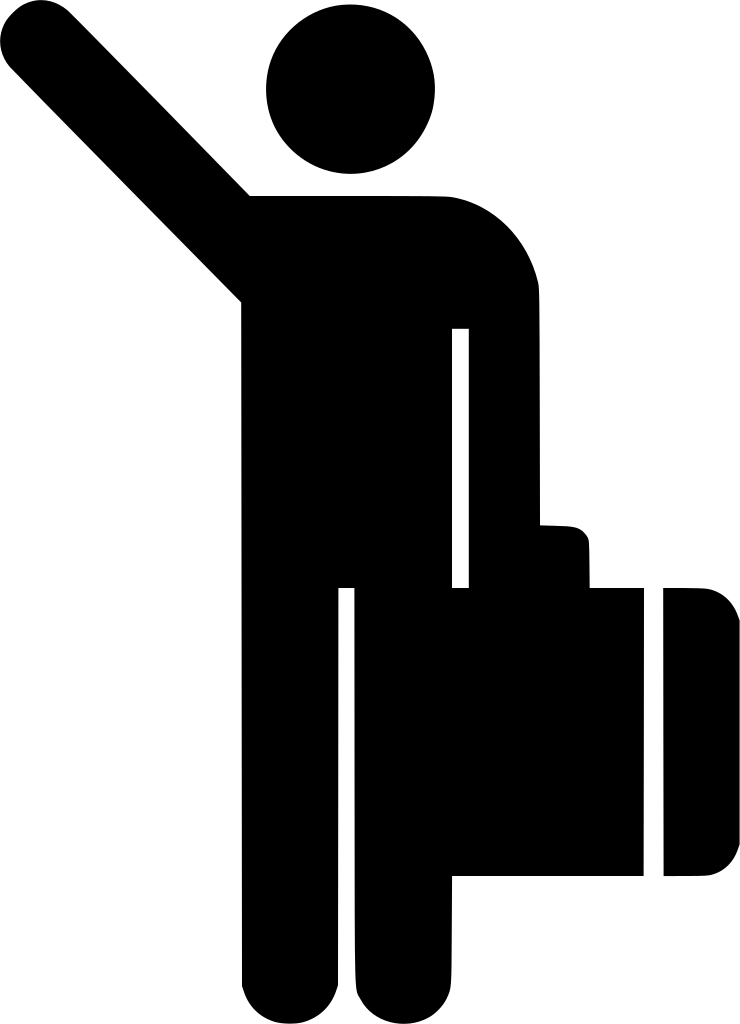
\includegraphics[width=0.5cm]{assets/img/client.png}} (place3);
        
        
        %\draw[->,] (place7) -- (place3) node[midway,above,sloped] {
\includegraphics[width=1cm]{assets/img/car.png} };
        \draw[->] (place6) -- node[midway, above, sloped] {
\includegraphics[width=1cm]{assets/img/car.png}} node[midway, above=0.8cm] {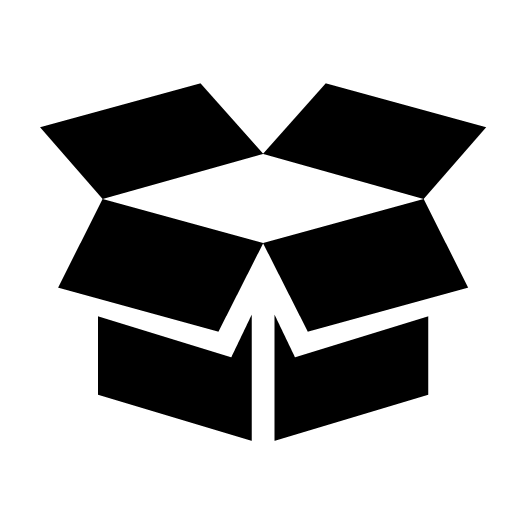
\includegraphics[width=0.5cm]{assets/img/goods.png}} (place7);
        
        % Define AVs nodes
        %\node[inner sep=0pt] (AV1) at (-2.25,0.5) {
\includegraphics[width=1cm]{assets/img/car.png}};
        %\node[inner sep=0pt] (AV2) at (0,0.5) {
\includegraphics[width=1cm]{assets/img/car.png}};
        %\node[inner sep=0pt] (AV3) at (2.25,0.5) {
\includegraphics[width=1cm]{assets/img/car.png}};
        
    \end{tikzpicture}
        
    }
\end{figure}
			}
			\only<3>{ % AV Rebalancing image
				\begin{figure}
    \resizebox{0.7\textwidth}{!}{
        \begin{tikzpicture}[>=stealth]
            % Define places nodes
            \node[circle, draw, minimum size=1.5cm] (place1) at (-3,2) { 1};
            \node[circle, draw, minimum size=1.5cm] (place2) at (0,2) { 2};
            \node[circle, draw, minimum size=1.5cm] (place3) at (3,2) { 3};
            \node[circle, draw, minimum size=1.5cm] (place4) at (-4,-1) { 4};
            \node[circle, draw, minimum size=1.5cm] (place5) at (-1,-1) { 5};
            \node[circle, draw, minimum size=1.5cm] (place6) at (1,-1) { 6};
            \node[circle, draw, minimum size=1.5cm] (place7) at (4,-1) { 7};
            
            % Arrows for roads
            %\draw[->] (place1) -- (place2);
            \draw[->] (place2) -- (place3);
            %\draw[->] (place1) -- (place4);
            \draw[->] (place4) -- (place5);
            \draw[->] (place5) -- (place6);
            \draw[->] (place6) -- (place7);
            \draw[->] (place7) -- (place3);
            
            \draw[->,] (place2) -- (place6) node[midway,above,sloped] {
\includegraphics[width=1cm]{assets/img/car.png} };
            
            
            \draw[->,] (place1) -- (place2) node[midway,above,sloped] {
\includegraphics[width=1cm]{assets/img/car.png} };
            
            
            
            \draw[->,] (place1) -- (place4) node[midway,above,sloped, xscale=-1] {
\includegraphics[width=1cm]{assets/img/car.png} };
            
            
            % Define AVs nodes
            %\node[inner sep=0pt] (AV1) at (-2.25,0.5) {
\includegraphics[width=1cm]{assets/img/car.png}};
            %\node[inner sep=0pt] (AV2) at (0,0.5) {
\includegraphics[width=1cm]{assets/img/car.png}};
            %\node[inner sep=0pt] (AV3) at (2.25,0.5) {
\includegraphics[width=1cm]{assets/img/car.png}};
            
        \end{tikzpicture}
        
    }
\end{figure}
			}
			\only<4>{ % Ride-Sharing image
				\begin{figure}
    \resizebox{0.9\textwidth}{!}{
        \begin{tikzpicture}[>=stealth]
            
            % Define clients nodes
            \node[inner sep=0pt] (client2) at (0,2.5) {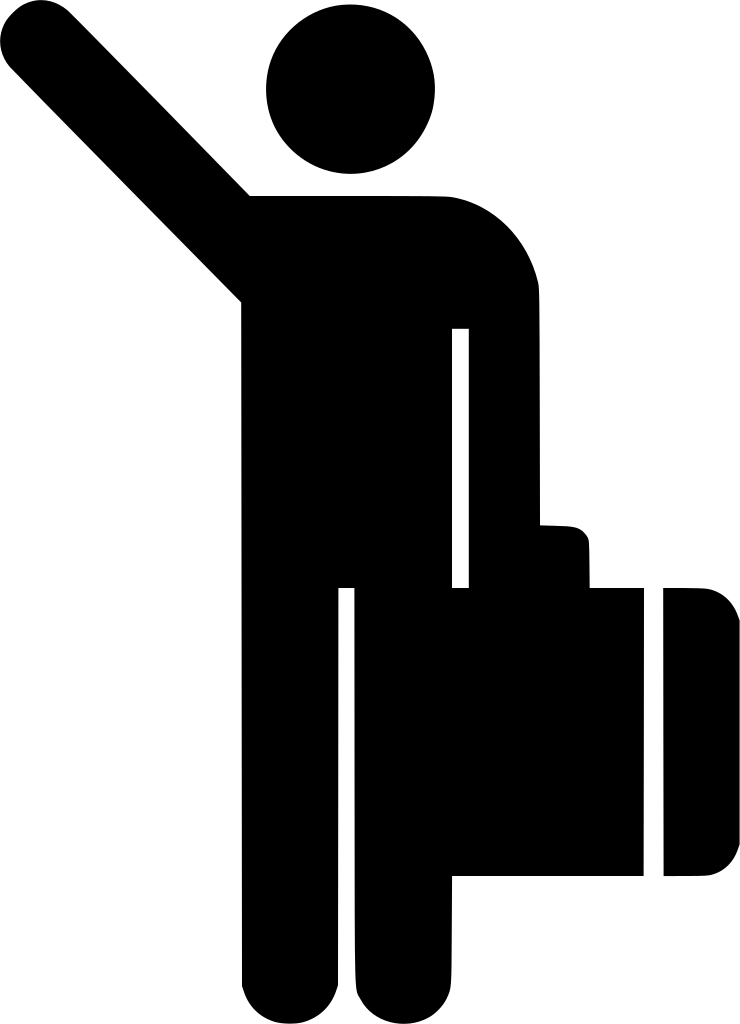
\includegraphics[width=1.1cm]{assets/img/client.png}};
            \node[inner sep=0pt] (client5) at (-1,0) {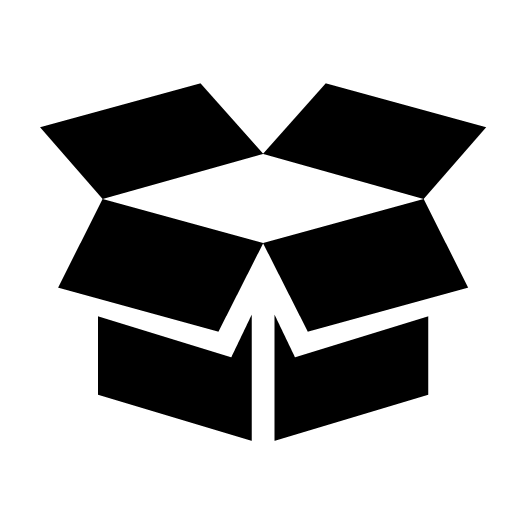
\includegraphics[width=1.1cm]{assets/img/goods.png}};
            \node[inner sep=0pt] (client6) at (1,0) {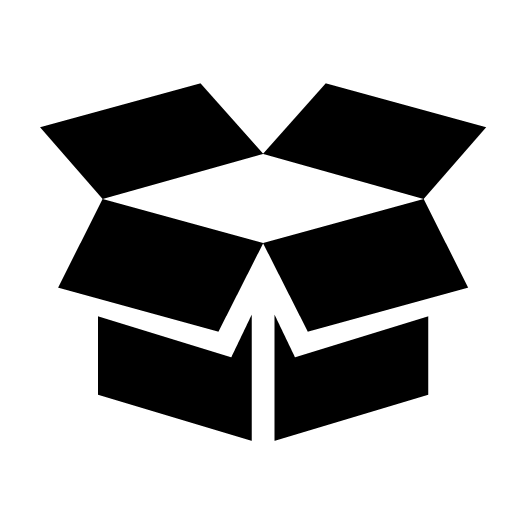
\includegraphics[width=1.1cm]{assets/img/goods.png}};
            
            % Define AVs nodes
            \node[inner sep=0pt] (AV2) at (0,-3) {
\includegraphics[width=2.4cm]{assets/img/car.png}};
            
            % Arrows from clients to AVs
            \draw[->] (client2.south) -- (AV2.north);
            \draw[->] (client5.south) -- (AV2.north);
            \draw[->] (client6.south) -- (AV2.north);
            
            % Label clients and AVs
            \node[above=0.2cm of client2] {Client 1};
            \node[above=0.2cm of client5] {Client 2};
            \node[above=0.2cm of client6] {Client 3};
            \node[below=0.2cm of AV2] {AV};
            
            \node[circle, draw, minimum size=1.5cm] (place1) at (5,1) { 1};
            \node[circle, draw, minimum size=1.5cm] (place2) at (8,1) { 2};
            \node[circle, draw, minimum size=1.5cm] (place3) at (11,1) { 3};
            \node[circle, draw, minimum size=1.5cm] (place7) at (13,-1) { 7};
            
            
            \draw[->] (place1) -- (place2);
            \draw[->] (place2) -- (place3);
            \draw[->] (place3) -- (place7);
            
            \node[left=0.2cm of place1, scale=4] {$\Rightarrow$};
            
            
            \node[inner sep=0pt] (client2a) at (place2)[above=1cm] { 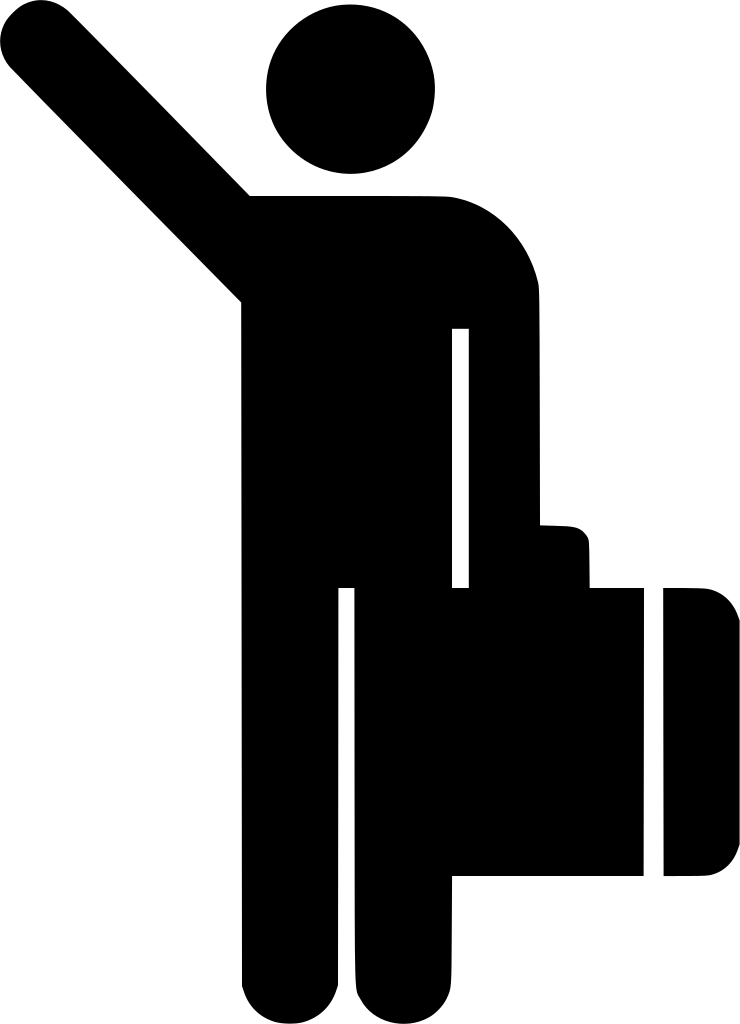
\includegraphics[width=1.1cm]{assets/img/client.png}};
            \node[inner sep=0pt] (client5a) at (place3)[above=1cm]{ 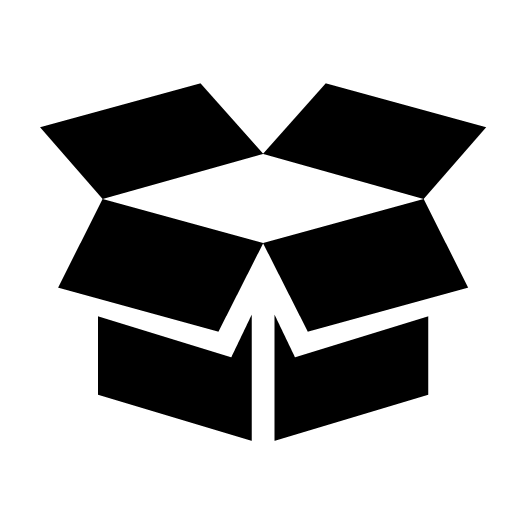
\includegraphics[width=1.1cm]{assets/img/goods.png}}; % Placed above place1
            \node[inner sep=0pt] (client6a) at (place7)[above=1cm]{ 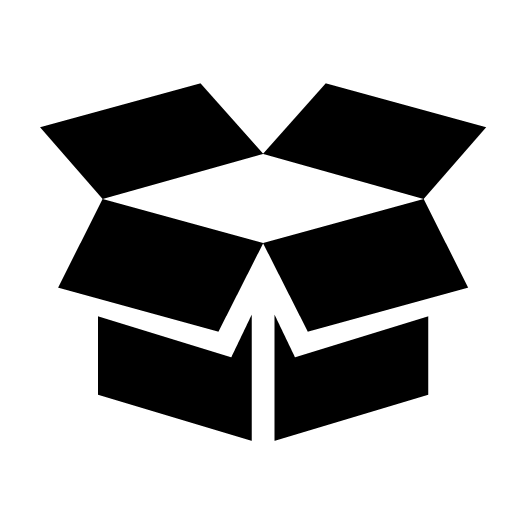
\includegraphics[width=1.1cm]{assets/img/goods.png}}; % Placed above place3
            \node[above=0.2cm of client2a] {Client 1};
            \node[above=0.2cm of client5a] {Client 2};
            \node[above=0.2cm of client6a] {Client 3};
        \end{tikzpicture}
        
    }
\end{figure}
			}
		\end{column}
	\end{columns}
\end{frame}


\section[Example 2]{Image next to text 2}



\begin{frame}{Tackling 4 Main Challenges}
	\begin{columns}
		\begin{column}{0.4\textwidth}
			
			\begin{itemize}
				\item \only<1>{\textbf{AV Dispatching}}\only<2->{AV Dispatching}
				\item \only<2>{\textbf{AV Routing}}\only<3->{AV Routing}
				\item \only<3>{\textbf{AV Rebalancing}}\only<4->{AV Rebalancing}
				\item \only<4>{\textbf{Ride-Sharing and Delivery Pooling}}
			\end{itemize}
				
		\end{column}
		%%
		\begin{column}{0.6\textwidth}
			\only<1>{ % AV Dispatching image
				\begin{figure}
    \resizebox{0.7\textwidth}{!}{
    \begin{tikzpicture}[>=stealth]
        
        % Define clients nodes
        \node[inner sep=0pt] (client1) at (-3,2.5) {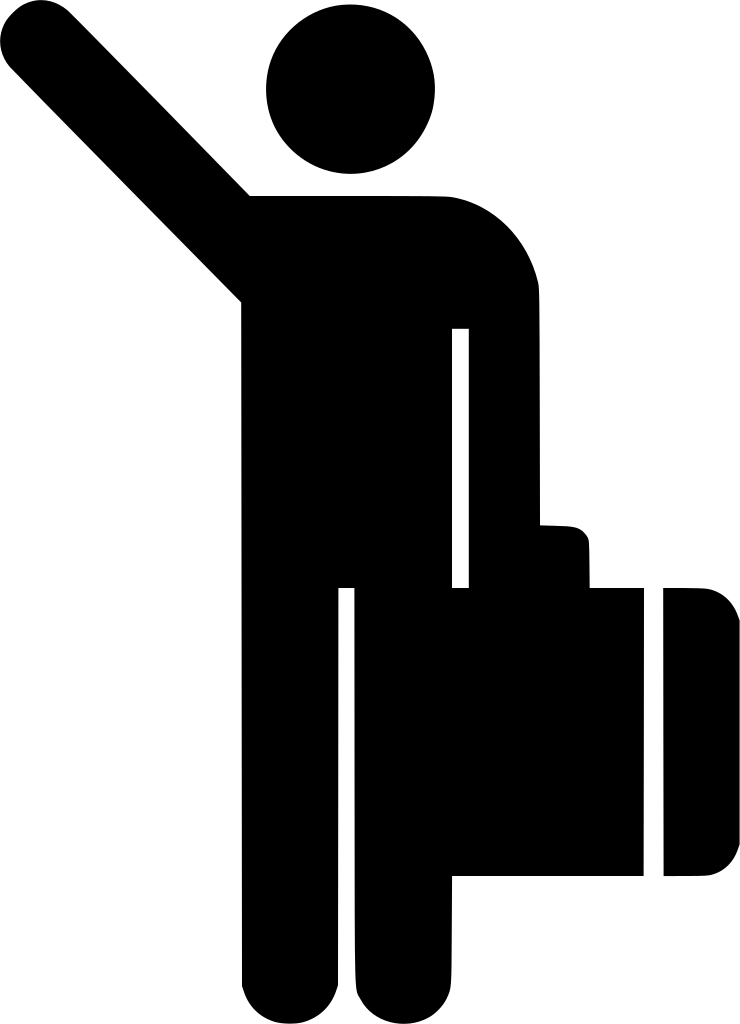
\includegraphics[width=1.1cm]{assets/img/client.png}};
        \node[inner sep=0pt] (client2) at (0,2.5) {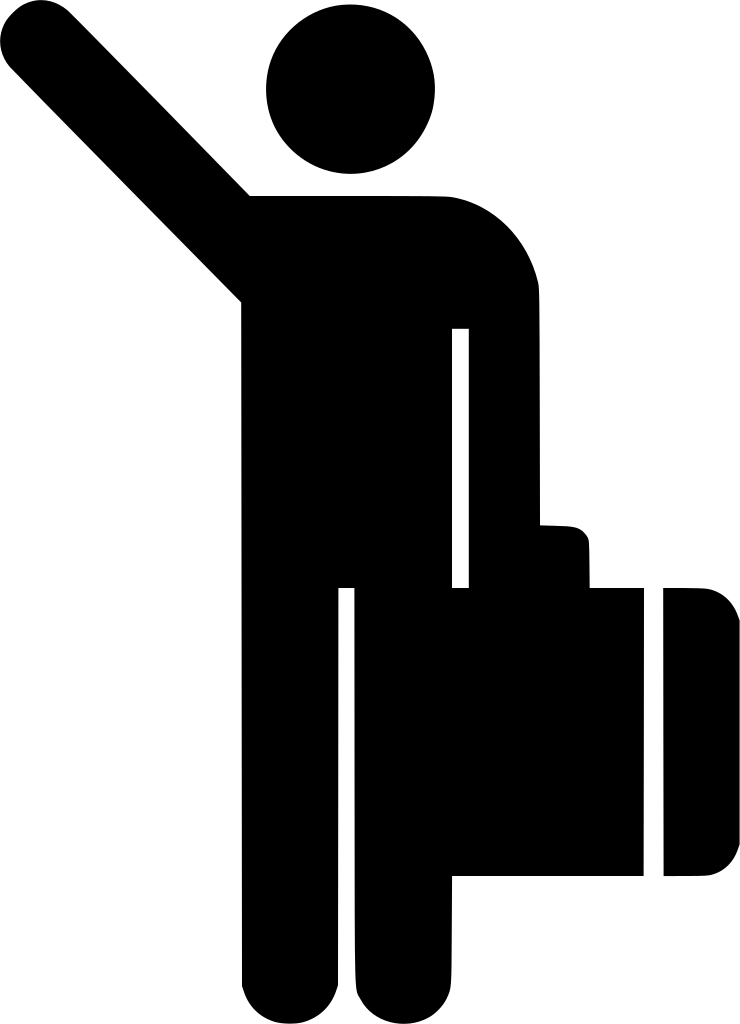
\includegraphics[width=1.1cm]{assets/img/client.png}};
        \node[inner sep=0pt] (client3) at (3,2.5) {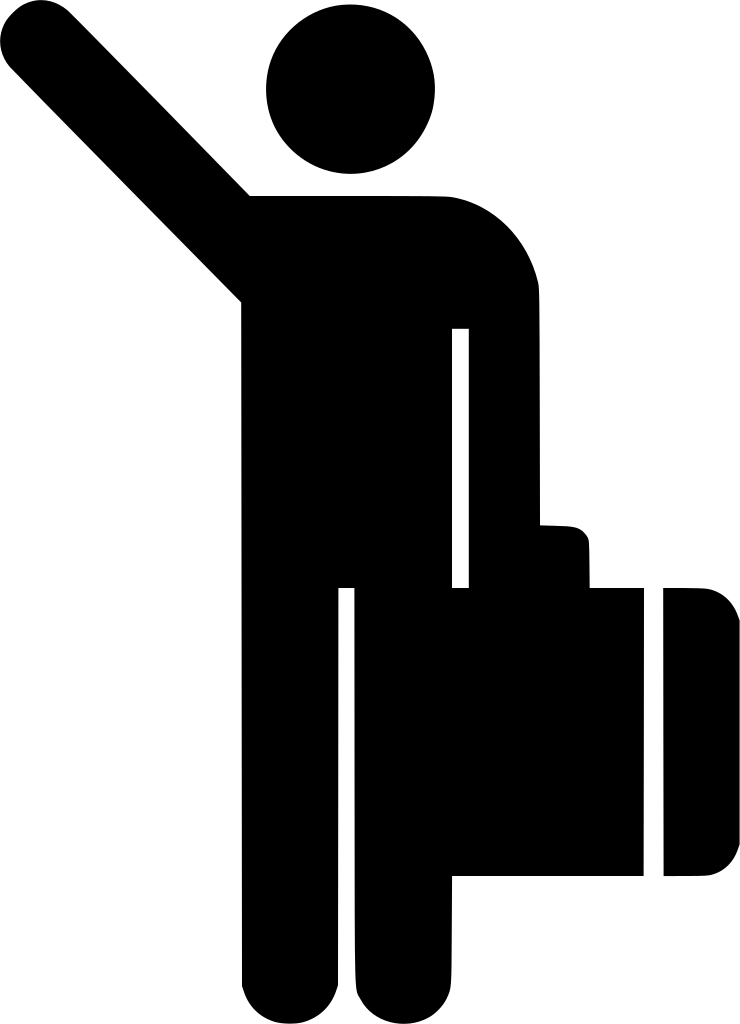
\includegraphics[width=1.1cm]{assets/img/client.png}};
        \node[inner sep=0pt] (client4) at (-4,0) {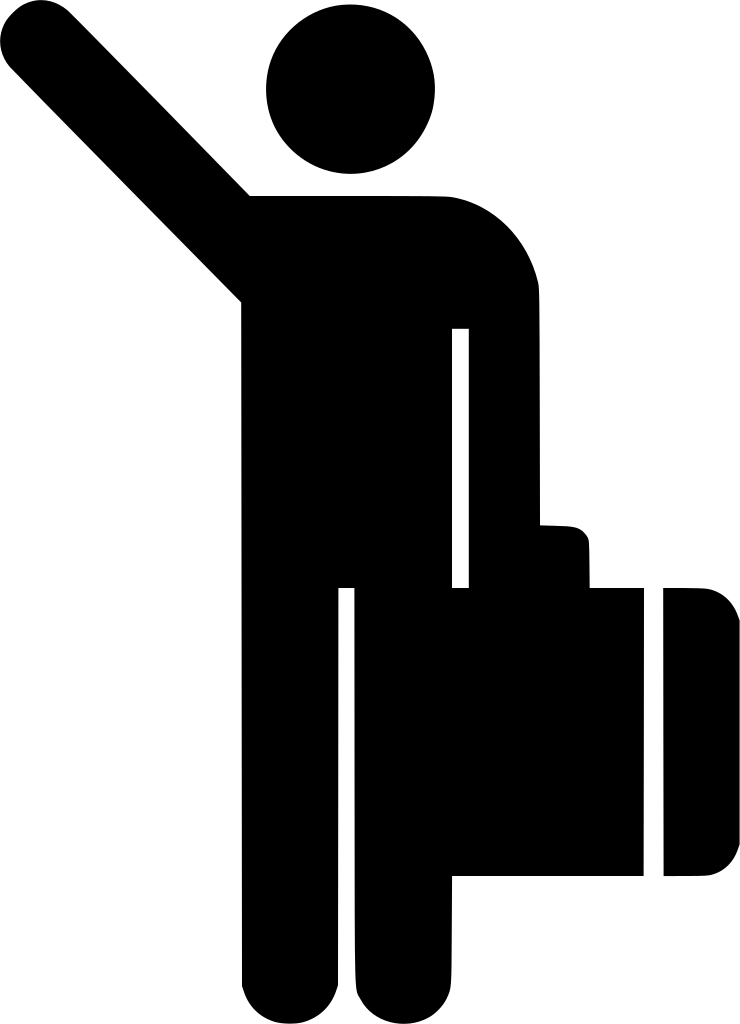
\includegraphics[width=1.1cm]{assets/img/client.png}};
        \node[inner sep=0pt] (client5) at (-1,0) {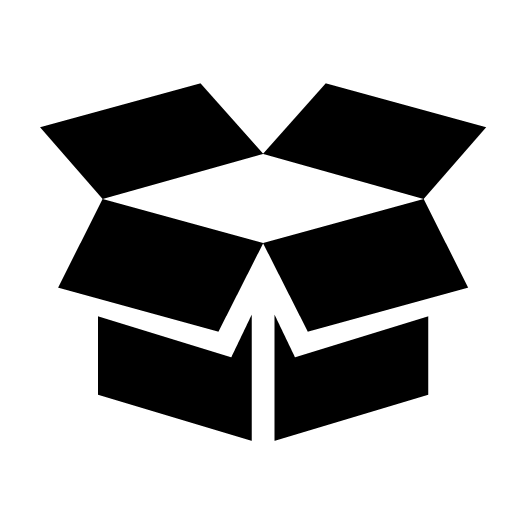
\includegraphics[width=1.1cm]{assets/img/goods.png}};
        \node[inner sep=0pt] (client6) at (1,0) {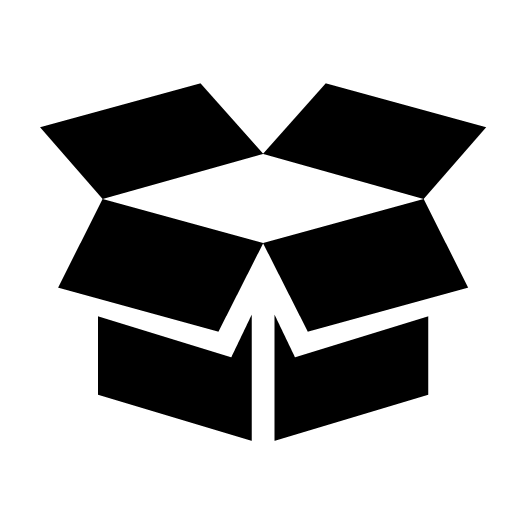
\includegraphics[width=1.1cm]{assets/img/goods.png}};
        \node[inner sep=0pt] (client7) at (4,0) {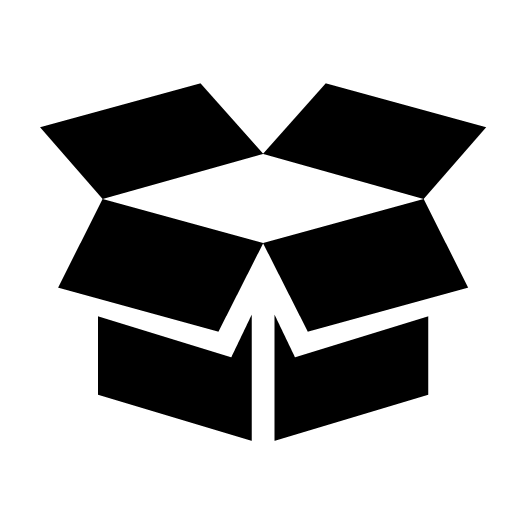
\includegraphics[width=1.1cm]{assets/img/goods.png}};
        
        % Define AVs nodes
        \node[inner sep=0pt] (AV1) at (-3,-3) {
\includegraphics[width=2.4cm]{assets/img/car.png}};
        \node[inner sep=0pt] (AV2) at (0,-3) {
\includegraphics[width=2.4cm]{assets/img/car.png}};
        \node[inner sep=0pt] (AV3) at (3,-3) {
\includegraphics[width=2.4cm]{assets/img/car.png}};

        
        % Arrows from clients to AVs
        \draw[->] (client1.south) -- (AV1.north);
        \draw[->] (client2.south) -- (AV2.north);
        \draw[->] (client3.south) -- (AV3.north);
        \draw[->] (client4.south) -- (AV1.north);
        \draw[->] (client5.south) -- (AV2.north);
        \draw[->] (client6.south) -- (AV2.north);
        \draw[->] (client7.south) -- (AV3.north);
        
        % Label clients and AVs
        \node[above=0.2cm of client1] {Client 1};
        \node[above=0.2cm of client2] {Client 2};
        \node[above=0.2cm of client3] {Client 3};
        \node[above=0.2cm of client4] {Client 4};
        \node[above=0.2cm of client5] {Client 5};
        \node[above=0.2cm of client6] {Client 6};
        \node[above=0.2cm of client7] {Client 7};
        \node[below=0.2cm of AV1] {AV 1};
        \node[below=0.2cm of AV2] {AV 2};
        \node[below=0.2cm of AV3] {AV 3};

        
    \end{tikzpicture}
    
}
\end{figure}
			}
			\only<2>{ % AV Routing image
				\begin{figure}
    \resizebox{0.9\textwidth}{!}{
    \begin{tikzpicture}[>=stealth]
        % Define places nodes
        \node[circle, draw, minimum size=1.5cm] (place1) at (-3,2) { 1};
        \node[circle, draw, minimum size=1.5cm] (place2) at (0,2) { 2};
        \node[circle, draw, minimum size=1.5cm] (place3) at (3,2) { 3};
        \node[circle, draw, minimum size=1.5cm] (place4) at (-4,-1) { 4};
        \node[circle, draw, minimum size=1.5cm] (place5) at (-1,-1) { 5};
        \node[circle, draw, minimum size=1.5cm] (place6) at (1,-1) { 6};
        \node[circle, draw, minimum size=1.5cm] (place7) at (4,-1) { 7};
        
        % Arrows for roads
        \draw[->] (place1) -- (place2);
        %\draw[->] (place2) -- (place3);
        \draw[->] (place1) -- (place4);
        %\draw[->] (place4) -- (place5);
        \draw[->] (place5) -- (place6);
        \draw[->] (place2) -- (place6);
        \draw[->] (place6) -- (place7);
        \draw[->] (place7) -- (place3);
        
        %\draw[->,] (place4) -- (place5) node[midway,above,sloped] {
\includegraphics[width=1cm]{assets/img/car.png} };
        \draw[->] (place4) -- node[midway, above, sloped] {
\includegraphics[width=1cm]{assets/img/car.png}} node[midway, above=0.8cm] {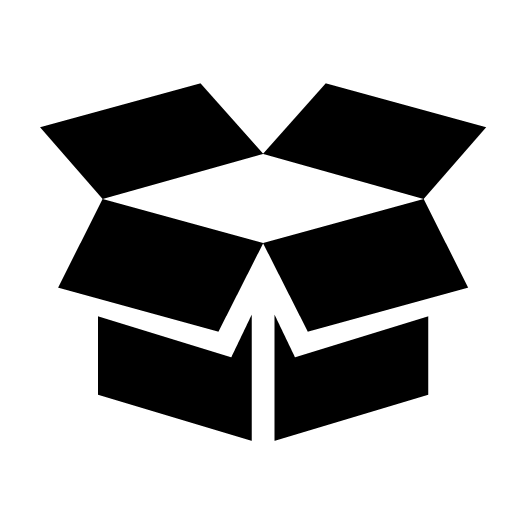
\includegraphics[width=0.5cm]{assets/img/goods.png}} (place5);
        
        %\draw[->,] (place2) -- (place3) node[midway,above,sloped] {
\includegraphics[width=1cm]{assets/img/car.png} };
        \draw[->] (place2) -- node[midway, above, sloped] {
\includegraphics[width=1cm]{assets/img/car.png}} node[midway, above=0.8cm] {\includegraphics[width=0.5cm]{assets/img/client.png}} (place3);
        
        
        %\draw[->,] (place7) -- (place3) node[midway,above,sloped] {\includegraphics[width=1cm]{assets/img/car.png} };
        \draw[->] (place6) -- node[midway, above, sloped] {\includegraphics[width=1cm]{assets/img/car.png}} node[midway, above=0.8cm] {\includegraphics[width=0.5cm]{assets/img/goods.png}} (place7);
        
        % Define AVs nodes
        %\node[inner sep=0pt] (AV1) at (-2.25,0.5) {\includegraphics[width=1cm]{assets/img/car.png}};
        %\node[inner sep=0pt] (AV2) at (0,0.5) {\includegraphics[width=1cm]{assets/img/car.png}};
        %\node[inner sep=0pt] (AV3) at (2.25,0.5) {\includegraphics[width=1cm]{assets/img/car.png}};
        
    \end{tikzpicture}
        
    }
\end{figure}
			}
			\only<3>{ % AV Rebalancing image
				\begin{figure}
    \resizebox{0.7\textwidth}{!}{
        \begin{tikzpicture}[>=stealth]
            % Define places nodes
            \node[circle, draw, minimum size=1.5cm] (place1) at (-3,2) { 1};
            \node[circle, draw, minimum size=1.5cm] (place2) at (0,2) { 2};
            \node[circle, draw, minimum size=1.5cm] (place3) at (3,2) { 3};
            \node[circle, draw, minimum size=1.5cm] (place4) at (-4,-1) { 4};
            \node[circle, draw, minimum size=1.5cm] (place5) at (-1,-1) { 5};
            \node[circle, draw, minimum size=1.5cm] (place6) at (1,-1) { 6};
            \node[circle, draw, minimum size=1.5cm] (place7) at (4,-1) { 7};
            
            % Arrows for roads
            %\draw[->] (place1) -- (place2);
            \draw[->] (place2) -- (place3);
            %\draw[->] (place1) -- (place4);
            \draw[->] (place4) -- (place5);
            \draw[->] (place5) -- (place6);
            \draw[->] (place6) -- (place7);
            \draw[->] (place7) -- (place3);
            
            \draw[->,] (place2) -- (place6) node[midway,above,sloped] {\includegraphics[width=1cm]{assets/img/car.png} };
            
            
            \draw[->,] (place1) -- (place2) node[midway,above,sloped] {\includegraphics[width=1cm]{assets/img/car.png} };
            
            
            
            \draw[->,] (place1) -- (place4) node[midway,above,sloped, xscale=-1] {\includegraphics[width=1cm]{assets/img/car.png} };
            
            
            % Define AVs nodes
            %\node[inner sep=0pt] (AV1) at (-2.25,0.5) {\includegraphics[width=1cm]{assets/img/car.png}};
            %\node[inner sep=0pt] (AV2) at (0,0.5) {\includegraphics[width=1cm]{assets/img/car.png}};
            %\node[inner sep=0pt] (AV3) at (2.25,0.5) {\includegraphics[width=1cm]{assets/img/car.png}};
            
        \end{tikzpicture}
        
    }
\end{figure}
			}
			\only<4>{ % Ride-Sharing image
				\begin{figure}
    \resizebox{0.9\textwidth}{!}{
        \begin{tikzpicture}[>=stealth]
            
            % Define clients nodes
            \node[inner sep=0pt] (client2) at (0,2.5) {\includegraphics[width=1.1cm]{assets/img/client.png}};
            \node[inner sep=0pt] (client5) at (-1,0) {\includegraphics[width=1.1cm]{assets/img/goods.png}};
            \node[inner sep=0pt] (client6) at (1,0) {\includegraphics[width=1.1cm]{assets/img/goods.png}};
            
            % Define AVs nodes
            \node[inner sep=0pt] (AV2) at (0,-3) {\includegraphics[width=2.4cm]{assets/img/car.png}};
            
            % Arrows from clients to AVs
            \draw[->] (client2.south) -- (AV2.north);
            \draw[->] (client5.south) -- (AV2.north);
            \draw[->] (client6.south) -- (AV2.north);
            
            % Label clients and AVs
            \node[above=0.2cm of client2] {Client 1};
            \node[above=0.2cm of client5] {Client 2};
            \node[above=0.2cm of client6] {Client 3};
            \node[below=0.2cm of AV2] {AV};
            
            \node[circle, draw, minimum size=1.5cm] (place1) at (5,1) { 1};
            \node[circle, draw, minimum size=1.5cm] (place2) at (8,1) { 2};
            \node[circle, draw, minimum size=1.5cm] (place3) at (11,1) { 3};
            \node[circle, draw, minimum size=1.5cm] (place7) at (13,-1) { 7};
            
            
            \draw[->] (place1) -- (place2);
            \draw[->] (place2) -- (place3);
            \draw[->] (place3) -- (place7);
            
            \node[left=0.2cm of place1, scale=4] {$\Rightarrow$};
            
            
            \node[inner sep=0pt] (client2a) at (place2)[above=1cm] { \includegraphics[width=1.1cm]{assets/img/client.png}};
            \node[inner sep=0pt] (client5a) at (place3)[above=1cm]{ \includegraphics[width=1.1cm]{assets/img/goods.png}}; % Placed above place1
            \node[inner sep=0pt] (client6a) at (place7)[above=1cm]{ \includegraphics[width=1.1cm]{assets/img/goods.png}}; % Placed above place3
            \node[above=0.2cm of client2a] {Client 1};
            \node[above=0.2cm of client5a] {Client 2};
            \node[above=0.2cm of client6a] {Client 3};
        \end{tikzpicture}
        
    }
\end{figure}
			}
		\end{column}
	\end{columns}
\end{frame}



\section[Example3]{Further examples}
\begin{frame}{A slide title}

  \begin{itemize}
    \item A bulleted item
    \item Another item
      \begin{itemize}
        \item With sub-bullets
        \item And another, with some \textbf{bold} text
      \end{itemize}
    \item And another, at the top level, with \textit{italic} text
  \end{itemize}

  \note{
    Here's a note for this slide.
  }

\end{frame}

\begin{frame}{A 50-50 split slide}

  \begin{columns}
    \begin{column}{0.5\linewidth}
      \begin{itemize}
        \item This side has a bullet
        \item And another bullet, with text that wraps if it's long
      \end{itemize}
    \end{column}
    \begin{column}{0.5\linewidth}
      \begin{figure}
        \centering
        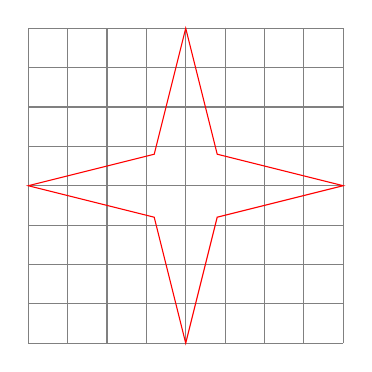
\begin{tikzpicture}[scale=2]
          \draw[step=0.25cm,color=gray] (-1,-1) grid (1,1);
          \draw[color=red] (1,0) -- (0.2,0.2) -- (0,1) -- (-0.2,0.2) -- (-1,0)
          -- (-0.2,-0.2) -- (0,-1) -- (0.2,-0.2) -- cycle;
        \end{tikzpicture}
        \caption{A figure caption}
      \end{figure}
    \end{column}
  \end{columns}

  \note{
    This slide has notes too.
  }

\end{frame}

\begin{frame}{Full-slide figure}

  \begin{figure}
    \centering
    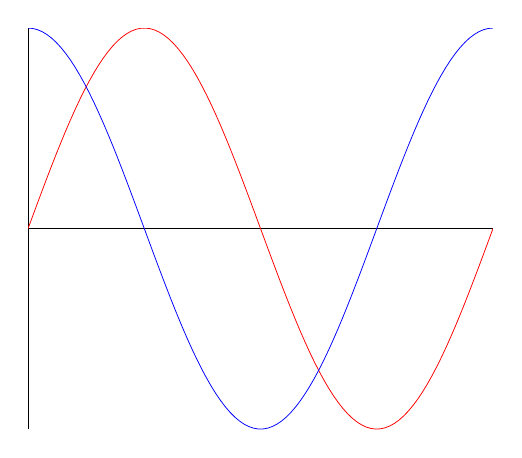
\begin{tikzpicture}[scale=0.7]
      \begin{axis}[
          scale only axis,
          no markers,
          domain=0:2*pi,
          samples=100,
          axis lines=center,
          axis line style={-},
          ticks=none]
        \addplot[red] {sin(deg(x))};
        \addplot[blue] {cos(deg(x))};
      \end{axis}
    \end{tikzpicture}
    \caption{The figure's caption}
  \end{figure}


\end{frame}


\begin{frame}{Full-slide sub-figure}

  \begin{figure}
  \begin{subfigure}[h]{0.45\textwidth}
    \centering
    \includegraphics[width=3cm]{assets/img/new_york_vanilla_info.png}
  \end{subfigure}
  \begin{subfigure}[h]{0.45\textwidth}
    \centering
    \includegraphics[width=3cm]{assets/img/new_york_simplified_roads.png}
  \end{subfigure}

   
  \end{figure}


\end{frame}
\begin{frame}{A slide with centered text}

  \begin{center}
    Some statement that is centered.
  \end{center}

  \vspace{2ex}
  \begin{center}
    \scriptsize (a small note)
  \end{center}

\end{frame}

\begin{frame}[fragile]{A slide with some code}

	\begin{columns}
		\begin{column}{0.5\linewidth}
			\footnotesize
			\begin{Verbatim}[commandchars=\\\{\}]
/* some code */
def foo(x):
  return x**0.5 + 2*x

\color{blue}/* some can be highlighted */
\color{blue}foo(3)
      \end{Verbatim}
    \end{column}
    \begin{column}{0.5\linewidth}
      {\color{red} Some explanatory text, in red, with some \texttt{monospace} text.}
      There might be some math, too:

      $$\sqrt{x} + 2x$$
    \end{column}
  \end{columns}

\end{frame}

\begin{frame}{A slide with some citations}

	\begin{itemize}
		\item Some statement {\cite{Brodo2022NNAnalysis}}
		\item Another statement {\cite{Brodo2022NNAnalysis}}
		\item A final statement {\cite{Brodo2022NNAnalysis}}
	\end{itemize}

	\vspace{3ex}
	\begin{center}
		\scriptsize (a small note)
	\end{center}

\end{frame}


\begin{frame}{A slide with some text and a link}

  \begin{itemize}
    \item This slide has some text along with a link
      \begin{itemize}
        \item \textbf{Some bold text}: followed by an explanation
        \item \textbf{More bold text}: followed by more text
      \end{itemize}
    \item Another bullet, with sub-bullets
      \begin{itemize}
        \item A sub-bullet
        \item Another sub-bullet, with more text
      \end{itemize}
  \end{itemize}

  \vspace{2ex}
  \begin{center}
    \color{blue} \href{https://github.com/lucabrodohshl/TeamHenklerTemplates}{Nice link}
  \end{center}

\end{frame}


\makebib{src/examplebib}

\end{document}